\documentclass[12pt,a4paper,openany]{report}

\usepackage[T1]{fontenc}
\usepackage[utf8]{inputenc}
\usepackage{lmodern}
\usepackage[portuguese,english]{babel}
\usepackage[a4paper,margin=25mm]{geometry}
\usepackage{graphicx}
\usepackage{booktabs}
\usepackage{tabularx}
\usepackage{array}
\usepackage{float}
\usepackage[font=small,labelfont=bf]{caption}
\usepackage{enumitem}
\usepackage{amsmath}
\usepackage{microtype}
\usepackage[nohyperlinks]{acronym}
\usepackage{etoolbox}
\patchcmd{\thebibliography}{\chapter*}{\section*}{}{}
\usepackage[hidelinks]{hyperref}
\makeatletter\g@addto@macro\UrlBreaks{\do\_}\makeatother

\graphicspath{{figures/}}
\newcolumntype{L}{>{\raggedright\arraybackslash}X}
\setlist{itemsep=2pt,topsep=4pt}
\renewcommand{\arraystretch}{1.15}

\begin{document}

%-------------------------------------------------------------- cover
\begin{titlepage}
  \centering
  \vspace*{2.5cm}
  {\LARGE Project 1 -- Abnormal EV Charging Sessions\par}
  \vspace{0.3cm}
  {\Large Task 1: Data Understanding, Audit and Preparation\par}
  \vspace{0.6cm}
  {\large Mestrado em Engenharia Informática\\
  Mineração de Dados (MINDD)\par}
  \vfill
  
\includegraphics[width=0.62\textwidth]{isep_logo.pdf}
  \vfill
  {\large \textbf{Estudantes:}\\
  Grupo XX\\
  Manuela Leite | 1200720@isep.ipp.pt\\
  {[Nome do colega]} | {[número]}@isep.ipp.pt\par}
  \vfill
  {\large Professor(a): {[Nome do professor]}\\
  Data: 04/10/2026\\
  Ano Letivo: 2026/2027\par}
  \vspace*{1cm}
\end{titlepage}

%-------------------------------------------------------------- front matter
\pagenumbering{roman}

\begin{otherlanguage}{portuguese}
\chapter*{Resumo}
Este relatório descreve a Tarefa 1 do Projeto 1: compreender, auditar e preparar 441\,077 sessões de
carregamento de veículos elétricos, com o objetivo de prever, no momento em que cada sessão começa, se
esta vai terminar de forma anormal. O ficheiro não traz o alvo. Derivámo-lo da causa de término e
validámo-lo contra as colunas de histórico do próprio conjunto de dados, obtendo 18,6\% de sessões
anormais.

Excluímos as oito colunas que só existem depois da sessão e um carimbo temporal de disponibilidade
duvidosa. Num diagnóstico, essas colunas fariam subir o PR-AUC de 0,604 para 0,834, um resultado
impossível de reproduzir em produção. Os dados não têm duplicados nem registos inválidos, e os valores em
falta são estruturais. O volume, a prevalência e o tipo de avaria mudam ao longo dos dois anos, pelo
que a avaliação é cronológica, com um período inicial excluído e purga das sessões cujo resultado ainda
não seria conhecido.

Retemos 29 variáveis em 7 grupos. Todas as operações que aprendem com os dados são ajustadas apenas no
período de treino. O histórico recente de avarias do posto de carregamento é o sinal mais forte.
\end{otherlanguage}

\chapter*{Abstract}
This report covers Task 1 of Project 1: understanding, auditing and preparing 441,077 electric-vehicle
charging sessions in order to predict, when each session starts, whether it will end abnormally. The file
does not contain the target. We derived it from the end cause and validated it against the dataset's own
history columns, which gives 18.6\% abnormal sessions.

We excluded the eight columns that only exist after the session and one timestamp whose availability is
doubtful. In a diagnostic, those columns would raise PR-AUC from 0.604 to 0.834, a result that could not
be reproduced in production. The data contain no duplicates and no invalid records, and the missing values
are structural. Volume, prevalence and fault type change over the two years, so evaluation is
chronological, with an excluded burn-in period and a purge of sessions whose outcome would not yet be
known.

We retain 29 features in 7 groups. Every operation that learns from the data is fitted on the training
period only. Recent failure history at the charging post is the strongest signal.

\tableofcontents
\listoffigures

\chapter*{Acronyms}
\begin{acronym}[ROC-AUC]
  \acro{AUC}{Area Under the Curve}
  \acro{BMS}{Battery Management System}
  \acro{EV}{Electric Vehicle}
  \acro{NaN}{Not a Number (missing value)}
  \acro{PCA}{Principal Component Analysis}
  \acro{PR-AUC}{Area under the Precision--Recall curve}
  \acro{PSI}{Population Stability Index}
  \acro{ROC-AUC}{Area under the Receiver Operating Characteristic curve}
  \acro{SMOTE}{Synthetic Minority Over-sampling Technique}
  \acro{VIF}{Variance Inflation Factor}
\end{acronym}

\cleardoublepage
\pagenumbering{arabic}

%-------------------------------------------------------------- 1
\chapter{Introduction}\label{ch:intro}

The goal is to predict, at the moment an EV charging session starts, whether it will end abnormally. Every
preparation decision answers two questions: would this information exist at that moment, and is it
trustworthy? The data are an educational adaptation of the China EV Charging Dataset \cite{zhang2025}:
441,077 sessions and 47 columns, from 31 Dec 2019 to 31 Dec 2021, at 92 charging posts in 13 stations and
3 districts of Jiaxing. The numbers come from the notebook
\nolinkurl{TP1_Task1_Merged.ipynb} (seed 42), and references of the form §x.y point to its sections.
References of the form C-§x.y point to the extended notebook
\nolinkurl{TP1_Task1_Data_Understanding_and_Preparation.ipynb}, which holds the model-based diagnostics
(feature-group ablation, class weights, cold-start scores) that move to Task 2.

\section{Target definition}\label{sec:target}

The file has no \texttt{is\_Abnormal} column, so we derive it from \texttt{end\_cause} (15 categories). The
dataset's pre-computed abnormal-count history columns were built from the true label, so we recomputed them
under three candidate mappings (Table~\ref{tab:target}, §5.2 for mappings A and B, C-§4.2 for all three). Only mapping A reproduces them. We adopt it,
pending the instructor's confirmation. The classes are about 4.4\,:\,1, so an ``always normal'' model
reaches 81\% accuracy, and accuracy is not an adequate metric.

\begin{table}[htbp]
  \centering\small
  \caption{Candidate definitions of the target and agreement with the history columns}
  \label{tab:target}
  \begin{tabularx}{\textwidth}{L>{\raggedright\arraybackslash}p{3.6cm}r}
    \toprule
    Definition of ``abnormal'' & Rows matching the supplied counts (6 windows) & Prevalence \\
    \midrule
    A. 13 fault causes (``Charging ends normally'' and ``User stops charging'' are normal) & $\geq$ 99.97\% in every window & 18.58\% \\
    B. Everything except ``Charging ends normally'' & 0.3--36\% & 53.93\% \\
    C. Charger faults only (vehicle-side faults count as normal) & 2--70\% & 12.11\% \\
    \bottomrule
  \end{tabularx}
\end{table}

%-------------------------------------------------------------- 2
\chapter{Data Audit and Exploration}\label{ch:audit}

\section{Availability at prediction time}\label{sec:leakage}

Seven post-hoc variables (energy, electricity cost, service charge, amount, actual payment, end time,
payment time) and \texttt{end\_cause} describe the result of the session, so we exclude them. On their own
they reach univariate ROC-AUC 0.82--0.85, above any legitimate variable (best 0.77,
Figure~\ref{fig:auc}). Adding them to the model raises PR-AUC from 0.604 to 0.834 (C-§15.3), which is the
optimistic, non-deployable result a leaky preparation would report. We also exclude \texttt{Order creation
time}: it is stamped after the start in 56\% of sessions and adds nothing measurable ($-0.003$ PR-AUC).

\begin{figure}[htbp]
  \centering
  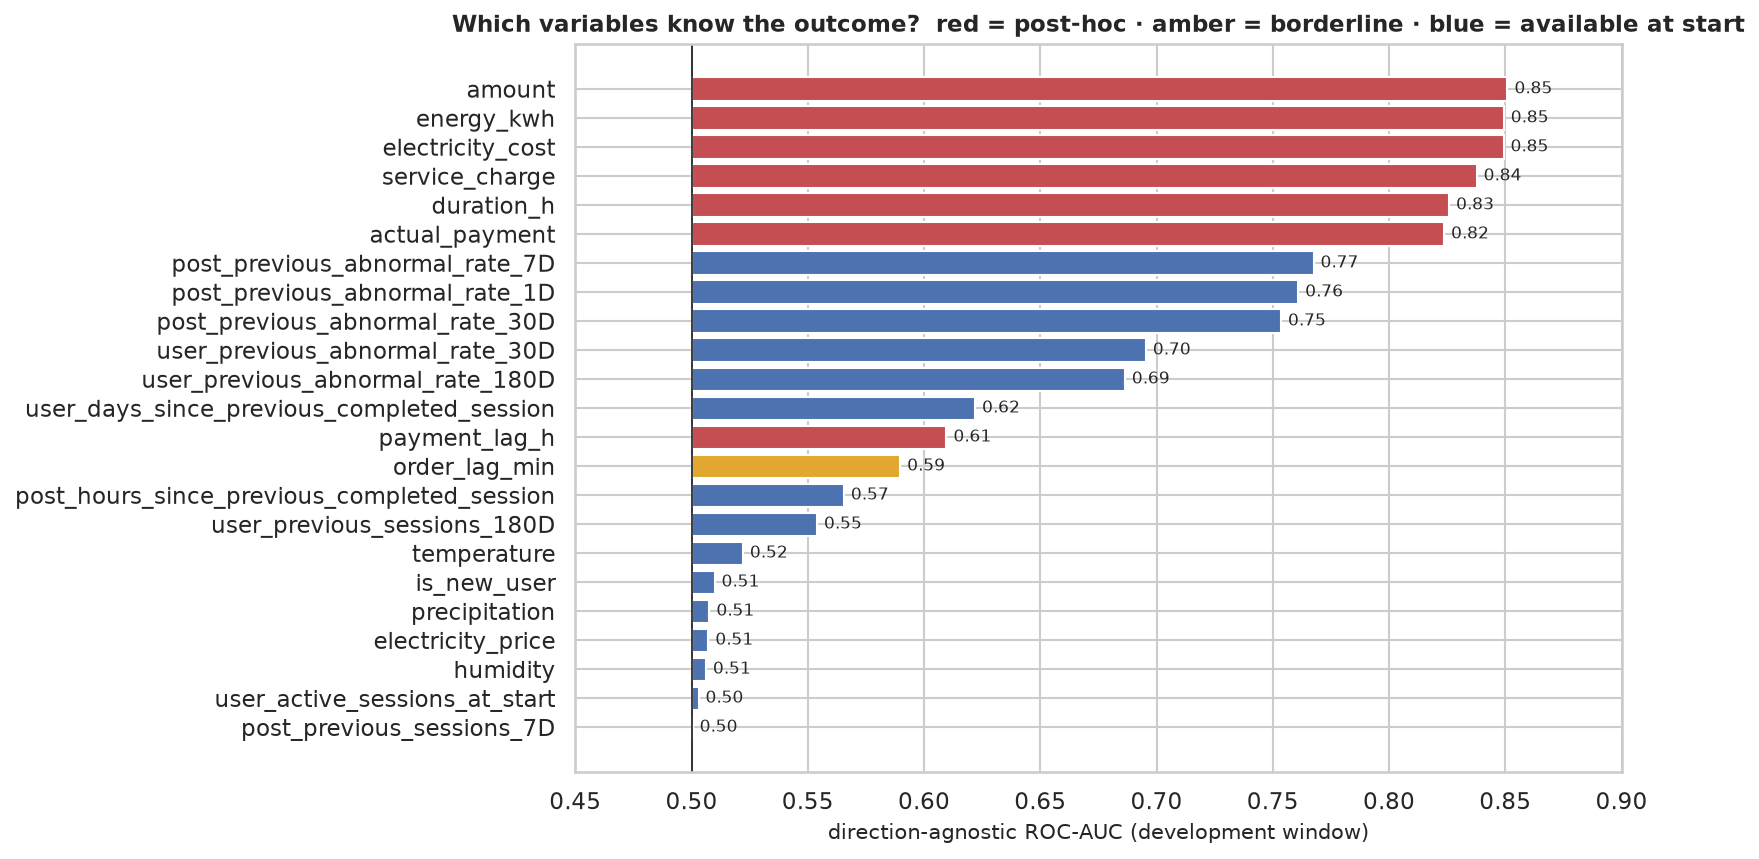
\includegraphics[width=0.85\textwidth]{06_1_univariate_auc_by_availability.png}
  \caption{Univariate ROC-AUC of each variable, coloured by availability at the start of the session}
  \label{fig:auc}
\end{figure}

\section{History attributes}\label{sec:history}

\textbf{Meaning.} Recomputing the history attributes from the timestamps reproduces the session counts in
at least 99.96\% of rows and the concurrency count in 99.97\% (C-§4.3). Only sessions that ended before the
current start are counted, so there is no look-ahead.

\textbf{Operational availability.} Post history needs a store that updates per-post counts when each
session ends, and the platform already records end causes. User history also needs the account to be
identified at start. Our validation and test values assume that this store is updated continuously.

\textbf{Privacy.} User history is a behavioural profile tied to a pseudonymous identifier. Removing it costs
0.037 PR-AUC, against 0.195 for post history (C-§15.1), so the modelling task will compare models with and
without it.

\textbf{Generalisation and cold start.} History replaces identities, so it works for accounts unseen in
training (40\% of validation and 61\% of test sessions). New accounts (about 13\% of sessions) get the
prior rate 0.2 and missing time-since values, and the model ranks them worse (C-§15.2). Post cold start
cannot be tested, because every validation and test post appears in training.

\section{Data quality}\label{sec:quality}

We removed no record and investigated each anomaly before deciding (Table~\ref{tab:quality}; §4, §6, §10).

\begin{table}[htbp]
  \centering\small
  \caption{Data-quality checks, findings and decisions}
  \label{tab:quality}
  \begin{tabularx}{\textwidth}{>{\raggedright\arraybackslash}p{2.5cm}LL}
    \toprule
    Check & Finding & Decision \\
    \midrule
    Duplicates & None (full rows or user + post + start) & No action \\
    Formatting & Trailing tab in 2 timestamp columns and 18,370 location values & Stripped on load \\
    Missing values & Only in the 4 ``time since previous'' columns; NaN equals the ``no previous'' flag in 100\% of rows & Structural, not imputed with mean or median; informative (14.4\% vs 19.3\% abnormal) \\
    Zero energy & 54,621 sessions, 45,563 of them abnormal & Kept: early faults and cancellations deliver no energy \\
    Post-hoc timestamps & Durations stop at 23.99\,h; 87,202 payments recorded before the end & Not used; censoring noted as a limitation \\
    Weather & One value per district and day & Treated as a forecast, as instructed (limitation) \\
    Outliers & Idle posts (39\% abnormal on return), fleet accounts, rainstorm days; Isolation Forest flags informative sessions & All kept; log and capping in the linear view only \\
    Cardinality & 92 posts, the smallest with 244 training sessions; fault causes from 20,114 down to 5 sessions & No grouping needed for a binary target \\
    \bottomrule
  \end{tabularx}
\end{table}

\section{What relates to abnormal termination}\label{sec:relations}

We measure relationships on the development window only (Apr 2020 to Jun 2021). The post matters most among
static variables: abnormal rates range from 4\% to 61\% across posts (Cramér's V 0.30, against 0.23 for
station and 0.11 for district), and post-level rates correlate at Spearman $\rho = 0.81$ between 2020 and
2021. Calendar and weather effects are small ($V \leq 0.042$). Recent failure history is the strongest
signal: the seven post-history variables top the univariate ranking (AUC 0.71--0.77) because faults cluster
in time at the same post (§9.4). The supplied rates are smoothed as (abnormal + 1) / (sessions + 5), so an
entity without history gets 0.2. Sessions concentrate in a few accounts (the top 1\% hold 34\%), so
\texttt{user\_id} is not usable and user history replaces it.

\section{Temporal stability}\label{sec:temporal}

The process is not stationary (Figure~\ref{fig:monthly}). Monthly volume falls to 1,391 sessions in
Feb 2020, coinciding with the COVID-19 restrictions, and reaches 25--28k in autumn 2021. Prevalence ranges
from 13.7\% to 26.3\% per month, and faulty-connection faults fall from 28\% of abnormal sessions in 2020Q1
to about 6\% from 2020Q3. 90--92 posts are active each month until posts 17--20 stop on 28 Sep 2021, and
active accounts grow from about 2,000 to 5,600--7,500 per month. The history attributes are censored at the
start of the file: 31\% of Jan 2020 sessions are flagged as new users (about 13\% later), and their PSI is
far above 0.25 in Q1-2020 and at most 0.10 from Q3-2020. A random split would mix these regimes and
overstate performance, so evaluation is chronological.

\begin{figure}[htbp]
  \centering
  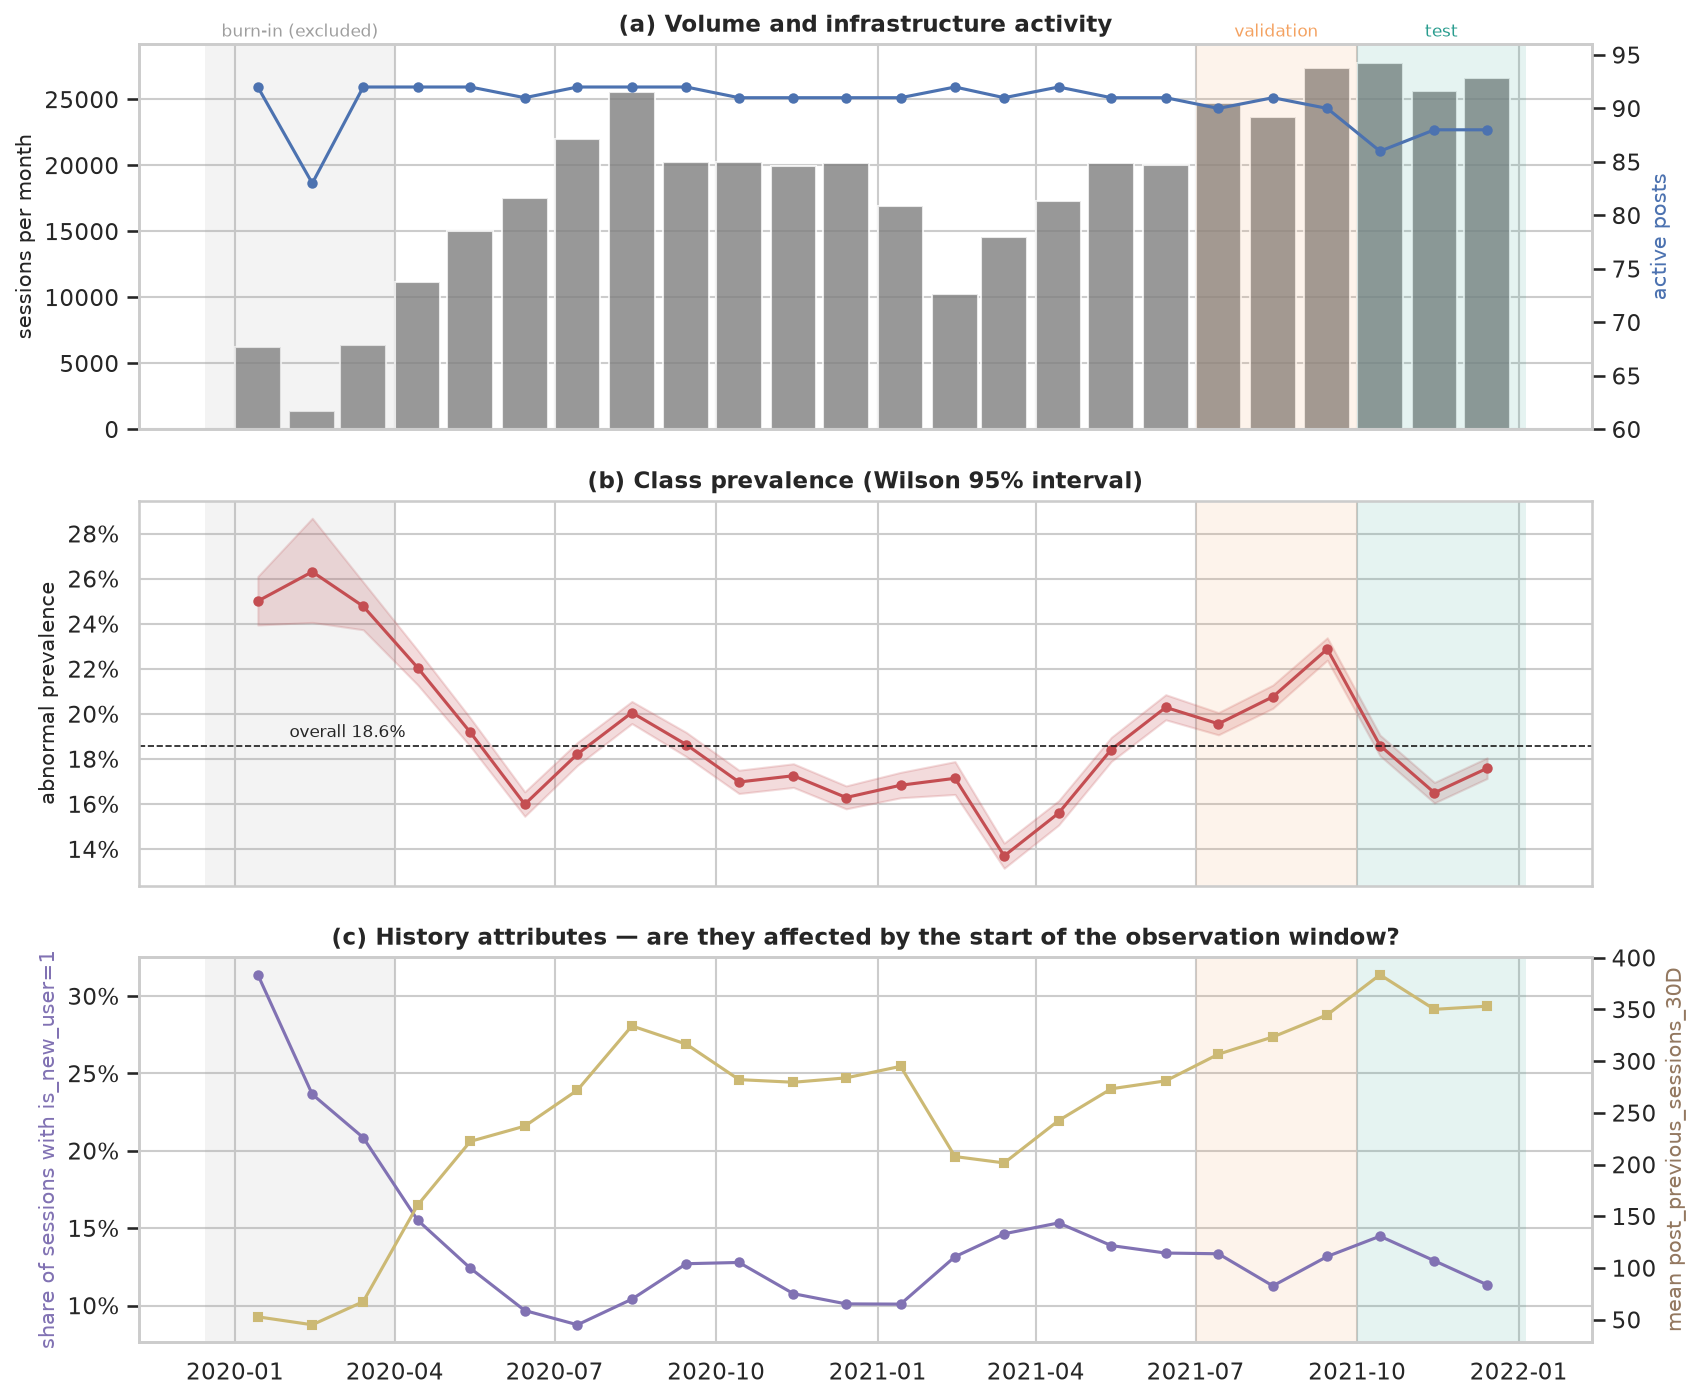
\includegraphics[width=\textwidth,height=0.45\textheight,keepaspectratio]{05_1_monthly_volume_prevalence_history.png}
  \caption{Monthly volume, abnormal rate and history availability}
  \label{fig:monthly}
\end{figure}

%-------------------------------------------------------------- 3
\chapter{Preparation and Evaluation}\label{ch:prep}

\section{Evaluation design}\label{sec:evaluation}

\begin{table}[htbp]
  \centering\small
  \caption{Chronological split}
  \label{tab:split}
  \begin{tabularx}{\textwidth}{>{\raggedright\arraybackslash}p{3.2cm}Lrr}
    \toprule
    Period & Dates & Sessions & Abnormal \\
    \midrule
    Burn-in (excluded) & 31 Dec 2019 to 31 Mar 2020 & 14,017 & 25.0\% \\
    Train & 1 Apr 2020 to 30 Jun 2021 & 271,182 & 17.8\% \\
    Purged & Train starts that end after 1 Jul 2021 & 28 & n/a \\
    Validation & Jul to Sep 2021 & 75,769 & 21.1\% \\
    Test (used once) & Oct to Dec 2021 & 80,081 & 17.6\% \\
    \bottomrule
  \end{tabularx}
\end{table}

Table~\ref{tab:split} shows the split. The burn-in is excluded because its history values are censored and
its fault regime is obsolete; including it changes PR-AUC by only $+0.0009$ (C-§15.4). Training rows must
also \emph{end} before the cutoff, since their label is unknown until then (purge). Hyper-parameters will be
tuned with three expanding-window folds inside the training period. We will report PR-AUC with lift over
the base rate, ROC-AUC, the Brier score, and precision and recall at a threshold chosen on validation.

\section{Retained features and learned operations}\label{sec:prep}

We retain 29 features in 7 groups: calendar (hour, day of week), tariff period, location
(\texttt{post\_id}, station, district), weather (4), post history (8), user history (10) and concurrency (1).
We drop \texttt{electricity\_price} (a function of the tariff), the six abnormal-count columns (exact
functions of counts and rates; adding them back changes nothing, C-§15.4), the post ``no history'' flags
(constant after the burn-in), \texttt{user\_no\_previous\_completed\_session} ($\phi \approx 1$ with
\texttt{is\_new\_user}), \texttt{is\_weekend} ($V = 0.001$) and \texttt{user\_id}.

Every operation that learns from data is fitted on the training period only, inside scikit-learn pipelines
(Table~\ref{tab:ledger}, C-§13). Fitting on all periods would change the parameters; for example, the
structural-NaN fill would move from 394 to 511 days. \texttt{log1p} and the sine/cosine encoding of hour and
weekday are stateless.

\begin{table}[htbp]
  \centering\small
  \caption{Learned operations, all fitted on the training period}
  \label{tab:ledger}
  \begin{tabularx}{\textwidth}{LLL}
    \toprule
    Operation & What is learned & Used by \\
    \midrule
    Category codes / one-hot (\texttt{post\_id}, station, district, tariff) & Category list & Tree / linear view \\
    Winsorisation of heavy-tailed variables & 0.1th and 99.9th percentiles & Linear view \\
    Structural-NaN fill (``never happened'') & Maximum; indicators kept & Linear view (trees keep NaN) \\
    Standardisation & Mean and standard deviation & Linear view \\
    Reduced numeric set (19 variables, max VIF 65 to 8.6) & Correlations on a training sample & Unregularised linear models \\
    Class-imbalance treatment & Class weights or resampling & Training folds only \\
    Rare-category grouping, PCA & Nothing & Not needed / not adopted \\
    \bottomrule
  \end{tabularx}
\end{table}

\section{Preliminary diagnostics}\label{sec:diagnostics}

A fixed, untuned gradient-boosting model on the training-window folds reaches PR-AUC 0.604 (folds
0.569--0.640; lift 3.56) and ROC-AUC 0.832. These runs check preparation decisions; they are not model
selection. Removing post history drops PR-AUC to 0.409, removing user history costs 0.037, and the other
groups, \texttt{post\_id} included, change it by at most 0.007 (Figure~\ref{fig:ablation}). Class weights
leave the ranking unchanged (0.602 vs 0.604) but push the mean prediction to 0.34 against a prevalence of
0.17, so the prepared data are not resampled and SMOTE is not used. For new accounts, ROC-AUC is 0.714
(lift 2.38), against 0.845 (lift 3.80) for returning users.

\begin{figure}[htbp]
  \centering
  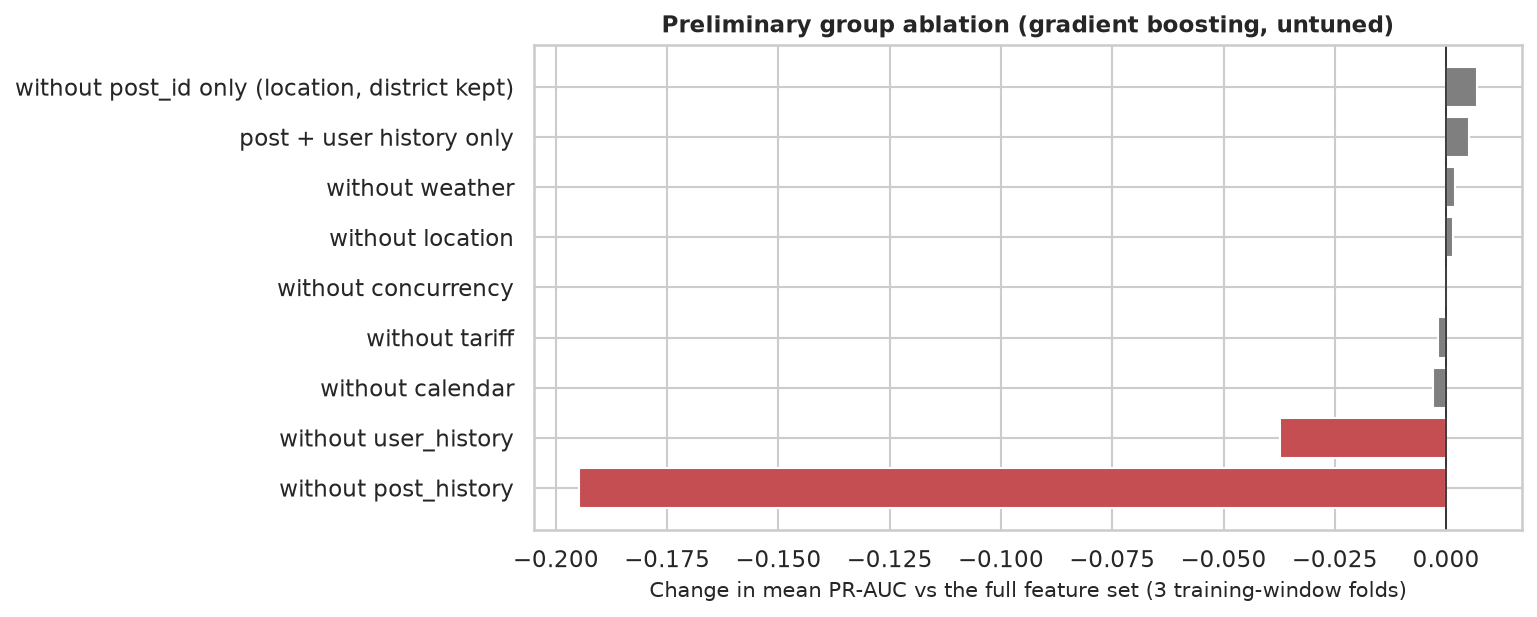
\includegraphics[width=0.75\textwidth]{15_1_group_ablation.png}
  \caption{Change in PR-AUC when each feature group is removed}
  \label{fig:ablation}
\end{figure}

%-------------------------------------------------------------- 4
\chapter{Synthesis}\label{ch:synthesis}

\begin{enumerate}[leftmargin=*,itemsep=4pt]
  \item \textbf{Main characteristics and problems.} The target had to be derived and validated (18.6\%
  abnormal). Eight outcome columns and one doubtful timestamp would leak it. Missing values are structural
  and no record is invalid. Volume, prevalence, fault mix and site mix drift, and history is censored in
  Q1-2020. Risk concentrates by post, and recent post failure history is the strongest signal.
  \item \textbf{Evidence for the decisions.} The history-count oracle (target), AUC and PR-AUC inflation
  (leakage), the 100\% match between NaN and its flag (missing values), the outlier investigation, PSI and
  monthly analyses (split), exact identities confirmed in C-§15.4 (redundancy), and the ledger of
  training-only parameters.
  \item \textbf{Retained variables.} 29 features in 7 groups. Post history is essential and user history is
  useful; the context groups remain candidates for the modelling task.
  \item \textbf{Limitations and assumptions.} The target mapping is inferred; weather is assumed to be a
  forecast but is daily; durations are censored at 24\,h; payment and order timing semantics are unknown;
  the causes of drift are hypotheses; post cold start cannot be tested; history in validation and test
  assumes a continuously updated store; fleet accounts dominate user counts; the diagnostics use one
  untuned model.
  \item \textbf{Implications for modelling.} Chronological split with purge, expanding-window
  cross-validation and a single use of the test set; PR-AUC with lift, ROC-AUC and calibration instead of
  accuracy; imbalance handled by the threshold or in-fold weights; tree ensembles and a regularised
  logistic-regression baseline; models compared with and without \texttt{post\_id} and user history, with
  cold-start users reported separately.
\end{enumerate}

%-------------------------------------------------------------- references
\begin{thebibliography}{9}
  \bibitem{zhang2025} Zhang, Y., Xu, T., Chen, T., et al. (2025). A high-resolution electric vehicle
  charging transaction dataset with multidimensional features in China. \emph{Scientific Data}, 12, 643.
  \url{https://doi.org/10.1038/s41597-025-04982-1}
\end{thebibliography}

\end{document}
